\documentclass[hyperref={pdfpagelabels=false}]{beamer}
\let\Tiny=\tiny
\hypersetup{pdfpagemode=FullScreen}
\usepackage[ngerman]{babel}
\usepackage[utf8]{inputenc}
\usepackage{graphics}
\usepackage{listings}
\usepackage{verbatim}
%\setbeamertemplate{navigation symbols}{}

\usetheme{Boadilla}

\usecolortheme{beaver}
\usefonttheme{professionalfonts}
\useinnertheme{rounded}
\useoutertheme{smoothbars}
%\useoutertheme{sidebar}

\author{Christian Kniep}

\begin{document}
\title[UNIX]{Advanced Operating System with UNIX}  
\institute[ICAT Bandung]{Internation Center of Applied Technologies Bandung}
\date[27.07.2010]{27. July 2010} 

\begin{frame}
	\titlepage
\end{frame} 

\begin{frame}
	\frametitle{Table of content}
	\tableofcontents
\end{frame} 


\section{Unit 2} 
	\subsection{Introduction to UNIX-Filesystem}
		\begin{frame}
			\frametitle{Introduction}
			\begin{itemize}
				\item<2-> There are only directorys or files, thats it!
                \item<3-> everything is a file, wether it is
                \begin{itemize}
                    \item<4-> a command, textfile, archive, etc.
                    \item<5-> a resources, setting
                \end{itemize}
                \item<6-> actually every file is a stream of byte, but lets skip that...
            \end{itemize}
		\end{frame}
    \subsection{Filesystem}
		\begin{frame}
			\frametitle{In General}
			\begin{itemize}
                \item<2-> The filesystem looks like a tree
				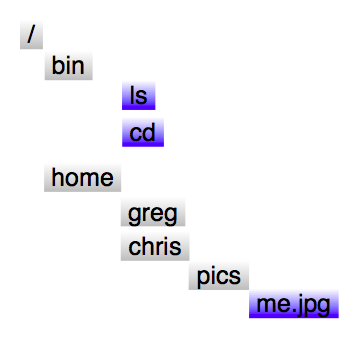
\includegraphics[height=0.5\columnwidth]{pics/fileSystem.png}<2>%
            \end{itemize}
		\end{frame}
		\begin{frame}
			\frametitle{In Detail}
			\begin{itemize}
                \item<2-> The basic folder-hierachie should be
				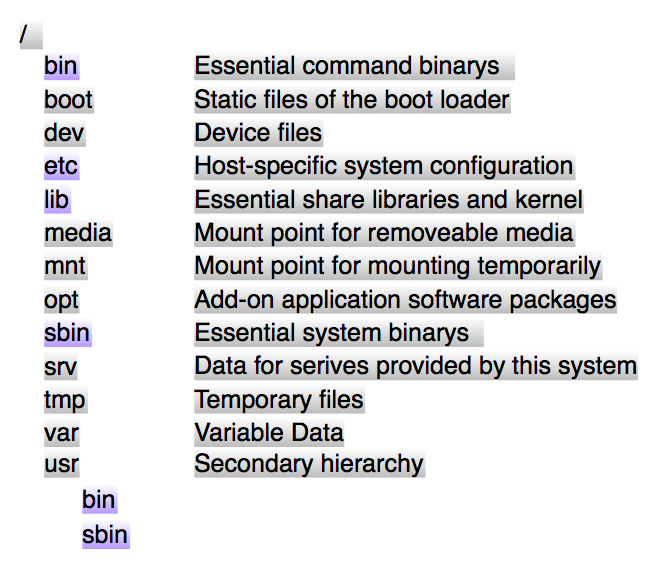
\includegraphics[height=0.5\columnwidth]{pics/fileSystemSM.png}<2>%
            \end{itemize}
		\end{frame}
	\subsection{Introduction to UNIX-Filesystem}
	    \begin{frame}
			\frametitle{File System Types 1}
			\begin{itemize}
                \item<1-> The Filesystem-Type defines how to use (speak to) the physical device
                \item<1-> There are several ones out there
                \begin{itemize}
                    \item<2-> historical types
                    \begin{itemize}
                        \item<2-> \textbf{s5}
                        \item<2-> \textbf{msdos},\textbf{pcfs}
                    \end{itemize}
                    \item<3-> to use windows-partitions
                    \begin{itemize}
                        \item<3-> \textbf{fat16},\textbf{fat32} the old Windows-Filesystem
                        \item<3-> \textbf{ntfs-3g} to support WindowsXP,Vista and 7
                    \end{itemize}
                \end{itemize}
            \end{itemize}
        \end{frame}
        \begin{frame}
			\frametitle{File System Types 2}
            \begin{itemize}
                \item<1-> not that common
                \begin{itemize}
                    \item<1-> \textbf{ufs(2)} for FreeBSD
                    \item<1-> \textbf{bfs} boot file system for SystemV
                \end{itemize}
                \item<2-> in broad use
                \begin{itemize}
                    \item<2-> \textbf{iso9660},\textbf{hsfs} for cdroms
                    \item<2-> \textbf{proc},\textbf{procfs} pseudo-FS in the memory to handle processes 
                    \item<2-> \textbf{ext2},\textbf{ext3} RedHat,debian-derivates
                    \item<2-> \textbf{xfs} SUSE 
                \end{itemize}
                \item<3-> upcomming
                \begin{itemize}
                    \item<3-> \textbf{ext4} due to long history of ext2,ext3
                    \item<3-> \textbf{zfs} pushed by sun, manage a consistant FS
                    \item<3-> \textbf{btfs} speak BetterFS, like ZFS but OpenSource
                \end{itemize}                
            \end{itemize}
		\end{frame}
    	\begin{frame}
			\frametitle{Swap? Whats that about?}
			\begin{itemize}
                \item<1-> If the memory is fully loaded the OS could outsource some process data to the swap partition
                \item<1-> a drawer (swap) in your desk (RAM) instead of the cabinet (filesystem)
                \item<2-> when the OS uses the swap we say 'the machine is swapping'
                \item<2-> very bad, because its way slower then the normal RAM!
            \end{itemize}
		\end{frame}
    	\begin{frame}
			\frametitle{Fdisk,mkfs}
			\begin{itemize}
                \item<1-> with fdisk you are able to create,alter and delete the partition-table
                \item<1-> new partitions could be set up with a filesystem by using mkfs
            \end{itemize}
		\end{frame}
    \subsection{Mount and Unmount}
	    \begin{frame}
			\frametitle{mount,umount}
			\begin{itemize}
                \item<1-> if you want a device be part of your 'File-System'-tree?
                \item<1-> use 'mount -t type device mountpoint' to do it
                \item<2-> if you want it to disapear use 'umount device' or 'umount mountpoint'
            \end{itemize}
		\end{frame}
    \subsection{Fsck: File System Checking}
	    \begin{frame}
			\frametitle{data errode to your fingertips}
			\begin{itemize}
                \item<1-> power blackout
                \item<1-> 'my dog bites on my pen-drive'
                \item<1-> you name it!
            \end{itemize}
        \end{frame}
        \begin{frame}
			\frametitle{it causes inconsistent states}
            \begin{itemize}
                \item<1-> multiple inodes claimes the same disk block
                \item<1-> a free block is not listed in the superblocks
                \item<1-> a used block is marked free
                \item<1-> ...
            \end{itemize}
		\end{frame}
        \begin{frame}
			\frametitle{soloution 'fsck'}
            \begin{itemize}
                \item<1-> Phase 1 (simple stuff)
                \begin{itemize}
                    \item<1-> Validates the inodes for correctness (format, block numbers)
                    \item<1-> declares blocks BAD (number out of Range), DUP (claimed by another inode)
                \end{itemize}
                \item<2-> Phase 2 (what files/directories are involved?)
                \begin{itemize}
                    \item<2-> Starting from root, \\
                              searches for OUT OF RANGE inode numbers detected in P1
                    \item<2-> found one, than removes the 'dir' or 'file'
                \end{itemize}
            \end{itemize}
        \end{frame}
        \begin{frame}
			\frametitle{soloution 'fsck'}
            \begin{itemize}
                \item<3-> Phase 3 (lost+founds)
                \begin{itemize}
                    \item<3-> Looking for unreferenced directories and stores their files in '$l+f$'
                    \item<3-> the files are named as the inode number
                \end{itemize}
                \item<1-> Phase 4 (check counter)
                \begin{itemize}
                    \item<1-> compares link count information from Phases 2 \& 3, correcting discrepancies
                \end{itemize}
            \end{itemize}
		\end{frame}

    \subsection{The Boot Procedure}
	    \begin{frame}
			\frametitle{Get it on}
			\begin{itemize}
                \item<1-> Hole process from pushing the button to have a login prompt
                \begin{itemize}
                    \item<2-> The memory-resident code
                    \item<2-> self-test
                    \item<3-> probes bus for boot device
                    \item<3-> Reading boot-sector from boot device
                    \item<4-> Boot-program reads kernel and initrd an passs control
                    \item<4-> Kernel identifies,initialise and configure the devices
                    \item<5-> Runs appropriate startup scripts (single- / multi-usermode)
                \end{itemize}
            \end{itemize}
		\end{frame}
	    \begin{frame}
			\frametitle{Get it on}
				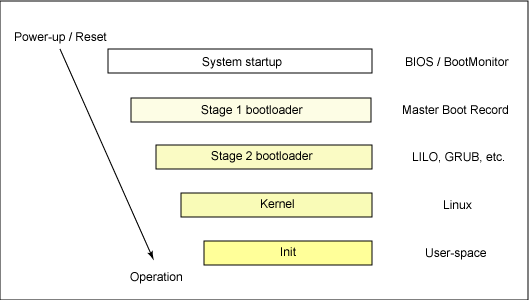
\includegraphics[height=0.5\columnwidth]{pics/startUp.png}<1>%
		\end{frame}
    \subsection{Kernel}
	    \begin{frame}
			\frametitle{Startup-process}
            \begin{itemize}
                \item<2-> The kernel ist kind of a puppetmaster who pulls the strings
                \item<2-> If he hadn`t initialise a device, it will not be available
            \end{itemize}
		\end{frame}
    \subsection{System Processes}
	    \begin{frame}
			\frametitle{What comes up?}
			\begin{itemize}
                \item<1-> To start the machine there are various processes that have to run
                \item<1-> the first process called 'swapper' it became PID 0 (but lives not long)
                \item<2-> the 2nd one is the init-Process (PID 1), which forks all the startup-scripts (init-scripts)
                \item<3-> on usual Unix-Systems the PID 2 is the first process created by the init-process and gets the PID 2
            \end{itemize}
		\end{frame}
	    \begin{frame}
			\frametitle{process table}
			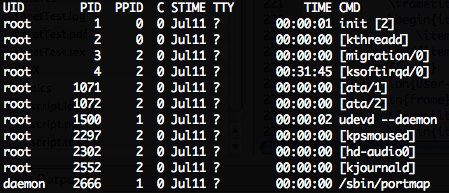
\includegraphics[height=0.4\columnwidth]{pics/ps.png}<1>%
		\end{frame}
    \subsection{Startup Scripts}
	    \begin{frame}
			\frametitle{As we are speaking of it...}
			\begin{itemize}
                \item<1-> the init-process (PID 1) are able to start scripts in various ways
                \item<1-> inittab (like in the SMU-book)
                \item<1-> Entry looks like '1:2345:respawn:/sbin/getty 38400 tty1'
                \item<2-> The entrys are 'id:runlevels:action:command'
                \begin{tabular}{lll}
                Entry & description \\
                id & Identifier \\
                runlevels & indicates in which runlevels the command should be started \\
                action & what action should be taken for this command, it may included: \\
                & sysinit & perform system initalization \\
                & wait & wait for the process to complete \\
                & once & run the process once only \\
                & respawn & restart the process whenever it dies \\
                commands & specifies the shell command to be run
                \end{tabular}
            \end{itemize}
		\end{frame}
    \subsection{User-/Group-Handling}
	    \begin{frame}
			\frametitle{Users}
			\begin{itemize}
                \item<2-> Will be used in Unit X
                \item<2-> useradd, adduser, usermod, chown
            \end{itemize}
		\end{frame}
	    \begin{frame}
			\frametitle{Groups}
			\begin{itemize}
                \item<2-> chgrp,addgroup
            \end{itemize}
		\end{frame}
    \subsection{Backup \& Restore}
	    \begin{frame}
			\frametitle{Backup \& Restore}
			\begin{itemize}
                \item<2-> 'dump, tar' vs 'rsync,dd'
            \end{itemize}
		\end{frame}



\end{document}